\chapter{How Bitcoin Works}

\begin{summary}
This chapter provides a high-level introduction of how Bitcoin works. It aims to be a summary of the prerequisite knowledge required by the reader before moving into the following chapters. The operation of the Bitcoin network is demonstrated with a walkthrough of a transaction and its journey from its creation up until its final destination, the Bitcoin blockchain.
\end{summary}

\section{The Story of a Transaction}
Transactions specify the transfer of bitcoin ownership. Assume we have three actors; Zed, Alice and Bob. Zed has sent 1.5 bitcoins to Alice with $TX_x$ and Alice wants to send 1 bitcoin to Bob. The transaction history will already have an entry of how Alice got her bitcoins (e.g. from Zed).

\begin{remark}
Internally, the Bitcoin protocol operates with satoshis: $1~satoshi = 0.00000001~BTC$. Thus, when we want to transfer 1 BTC we actually transfer $100000000~satoshis$.
\end{remark}

To send 1 bitcoin (or \emph{BTC}) Alice needs to create a transaction $TX_y$ that sends 1 BTC to Bob. We know that Alice has at least 1.5 BTC from $TX_x$.

\begin{emphbox}
\begin{lstlisting}
    $TX_x$: 1Zed transfers 1.5 BTC to 1Alice
    $TX_y$: 1Alice transfers 1 BTC to 1Bob
\end{lstlisting}
\end{emphbox}

The names 1Zed, 1Alice and 1Bob are short for the actual bitcoin addresses of Zed, Alice and Bob respectively. So Alice will send 1 BTC from her 1Alice bitcoin address to Bob to his 1Bob address.

Alice has to prove that she is indeed the owner of the address 1Alice when she creates the $TX_y$. Bob does not need to do anything to receive the bitcoins.

A transaction can consist of several \textbf{\emph{inputs}} (addresses to get bitcoins from\footnote{This is an oversimplification. In reality unspent outputs or UTXOs are used as inputs which are associated with an address.}) and several \textbf{\emph{outputs}} (addresses to send bitcoins to). When an input is used it is completely consumed; i.e. all the bitcoins that the TX contains as inputs need to be \textbf{\emph{spent}}.

\begin{figure}[h]
\begin{center}
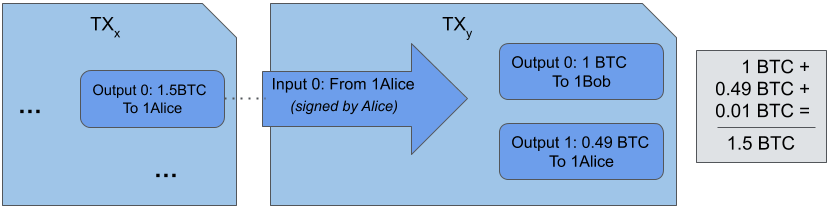
\includegraphics[scale=0.5]{images/typical-transaction}
\caption{Typical one input two outputs transaction.}
\label{fig:typical-transaction}
\end{center}
\end{figure}

The amount of all the inputs needs to be greater or equal to the amounts of outputs. If greater (recommended) the difference is an implied transaction fee that goes to the miners (see figure~\ref{fig:typical-transaction}). A typical transaction transfers some bitcoins to another user and returns the remaining bitcoins as change to the originating address or another address that the sender controls.

\begin{remark}
For privacy reasons it is recommended to send the change to a different address than the originating. Most bitcoin wallets already do this behind the scenes.
\end{remark}

Any number of inputs and outputs is possible as long as a transaction fee is included; the larger the transaction the larger the transaction fee. The unspent outputs are called \emph{Unspent Transaction Outputs (UTXOs)} and the set of UTXOs is essentially all the available bitcoins in the network.

Once a transaction is created it needs to be sent to a Bitcoin node. After the node receives the transaction it checks if it is valid, e.g. the output amounts should be less or equal to the input amounts, the signature proving ownership should be valid, etc. If it is valid the node will propagate it to all its peers\footnote{To be more precise they will notify their peers of the transaction by its \emph{transaction identifier (txid)} and the peers can choose to request it or not. More details will be provided in the Peer-to-Peer chapter.}, i.e. the other nodes that it is aware of. In turn, the other nodes will check if the transaction is valid and so on and so forth until all nodes receive the transaction (see figure~\ref{fig:transaction-propagation}).

\begin{figure}[h]
\begin{center}
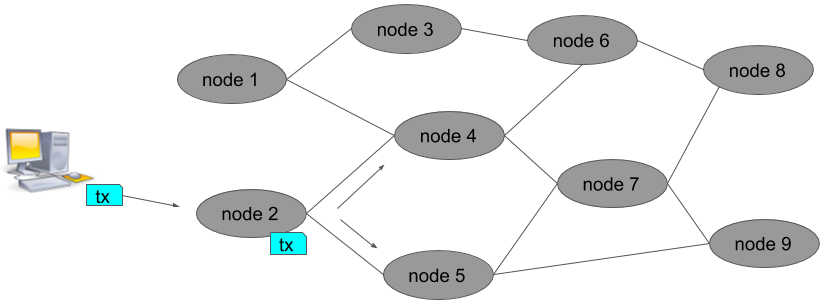
\includegraphics[scale=0.5]{images/transaction-propagation}
\caption{Transaction propagation through the network example.}
\label{fig:transaction-propagation}
\end{center}
\end{figure}


\section{From Transactions to Blocks}
From a Bitcoin's node perspective, the node receives transactions and places all valid ones into its memory pool, or \emph{mempool}. It keeps receiving new ones until it decides that it will group some of those transactions into a block (see figure~\ref{fig:node-perspective}).

\begin{figure}[h]
\begin{center}
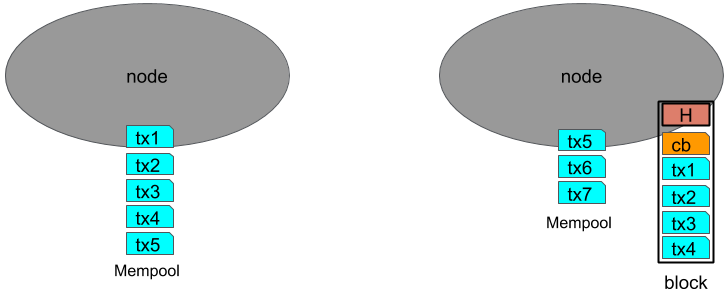
\includegraphics[scale=0.5]{images/node-perspective}
\caption{A node receives transactions into its mempool and can attempt to create new blocks for the network.}
\label{fig:node-perspective}
\end{center}
\end{figure}

\vspace{3em}
\begin{remark}
We are describing what mining nodes typically do. The majority of nodes are not mining nodes and thus do not attempt to create new blocks, rather they validate and propagate valid transactions and blocks when they are aware of them.
\end{remark}

Every block contains a \emph{coinbase} transaction that is added by the miner (see next section) and it sends a deterministically calculated reward to an address of the miner's choosing. Finally a header is added to the block containing important information that links this block to its parent and other information that we will examine in the next section.

\section{Mining}
After a node creates a block it will attempt to make it final by propagating it to all other nodes in the network. Multiple nodes will receive the same transactions and will create blocks; nodes choose which TXs to include (see figure~\ref{fig:different-nodes-mining}). They can create and propagate a block at any time.

\begin{emphbox}
But how do we select which blocks will be part of the blockchain? Since, miners include a reward for themselves everyone wants their block to be the next block in the blockchain. In other words, how do we avoid spam and Denial of Service (DoS) attacks?
\end{emphbox}

For a block to be considered valid a miner has to prove that he has done some intensive computational work. Thus, miners have to spend resources before they create a block. This mechanism of proving computational work is called \emph{Proof-of-Work (PoW)} and it involves solving a problem or puzzle. PoW puzzles have the fundamental property of being difficult to solve but trivial to validate their correctness. 

Bitcoin mining is the process of solving the PoW puzzle and selecting the next valid block in a way that is undisputed and thus achieve consensus on the current blockchain state. Bitcoin uses the Hashcash PoW algorithm~\cite{Back2002-hashcash} for its mining.

\begin{figure}[h]
\begin{center}
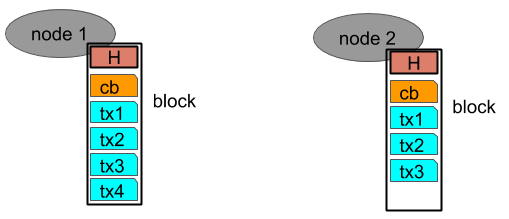
\includegraphics[scale=0.5]{images/different-nodes-mining}
\caption{All nodes will eventually receive all transactions but they are free to include them into a block as they see fit.}
\label{fig:different-nodes-mining}
\end{center}
\end{figure}

The Proof-of-Work puzzle is to compute a cryptographic hash of the new block that we want to create which should be less than a given number. The target number that the hash needs to be less than can be deterministically calculated by all nodes and is such that it would take around 10 minutes to calculate with the current network processing power, also called hashing power. Since a hash is random it will take several attempts to find a proper hash but other nodes will verify with only one attempt.

\begin{remark}
A cryptographic hash function is a hash function that takes an arbitrary block of data and returns a fixed-size bit string, the cryptographic hash value, such that any (accidental or intentional) change to the data will also change the hash value significantly.
\end{remark}

As more miners join the blocks will be created faster so the puzzle’s difficulty automatically adjusts (increases) so that it again requires approximately 10 minutes to solve. This \emph{difficulty adjustment} is happening every 2016 blocks, which is approximately 2 weeks if each block takes 10 minutes to mine.

The hash algorithm used is $SHA256$ and it is applied twice to the block header. As we will see later the header uniquely represents the whole block including all the transaction and thus hashing the header is effectively the same as hashing the whole block but with the added benefit of efficiency since the header is much smaller.

\begin{emphbox}
\begin{lstlisting}
SHA256( SHA256( block_header ) )
\end{lstlisting}
\end{emphbox}

The miner that successfully creates a valid block first will get the bitcoin reward that they have set themselves in the coinbase transaction as well as the fees from all the transactions in the block.

The block reward can be deterministally calculated according to the current \emph{block height}. The reward started at 50 bitcoins and is halved every 210000 blocks (approximately 4 years for 10 minute blocks). So, after block 630000 the reward will be 6.25 bitcoins. The mining reward can be claimed by the miner only after 100 \emph{confirmations}, i.e. after 100 blocks have been confirmed as part of the blockchain since.




\section{Blocks and Nakamoto Consensus}
If the transaction does not make it into a block it remains in the mempool to be added into the next block. If the node is made aware of a new valid block then it updates the block th
\section{Basic interaction with a node}

%problems? exercises? computer excercises???

